I test sono stati effettuati su un dataset da 10000 fino a 10000000 email, con una probabilità di falsi positivi di
0.10, 0.05 e 0.01.
Le email sono state generate casualmente tramite le funzioni contenute
Poiché i test variano da 10000 a 10000000 email, il numero di funzioni hash e la dimensione del vettore di bit sono
rispettivamente 5, e da un minimo di 62353 a un massimo di 62352243.

\subsection{OpenMP}\label{subsec:openmp-test}
\subsubsection{Setup}\label{subsubsec:openmp-setup}
\begin{figure}[H]
    \centering
    \minipage{0.49\textwidth}
    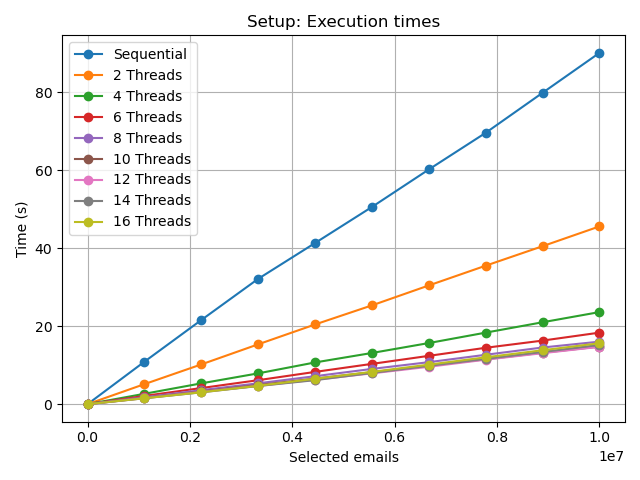
\includegraphics[width=\linewidth]{openmp/005/setup_times}
        \caption{Time setup Omp}\label{fig:005-setup_time_omp}
    \endminipage\hfill
    \minipage{0.49\textwidth}
    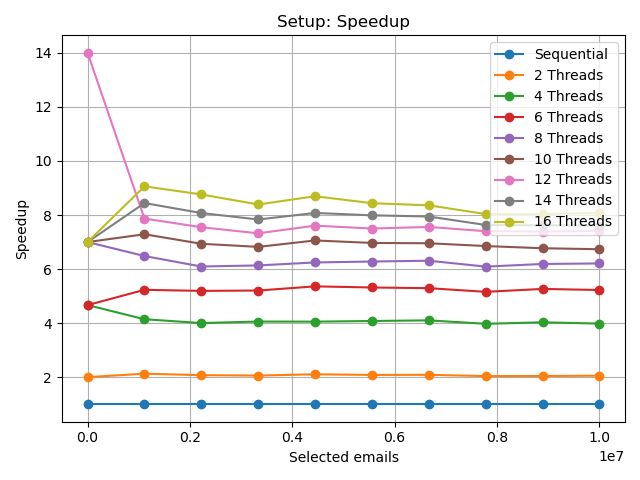
\includegraphics[width=\linewidth]{openmp/005/setup_speedup}
        \caption{Speedup setup Omp}\label{fig:005-setup_speedup_omp}
    \endminipage\hfill
\end{figure}
\begin{figure}[H]
    \centering
    \minipage{0.49\textwidth}
    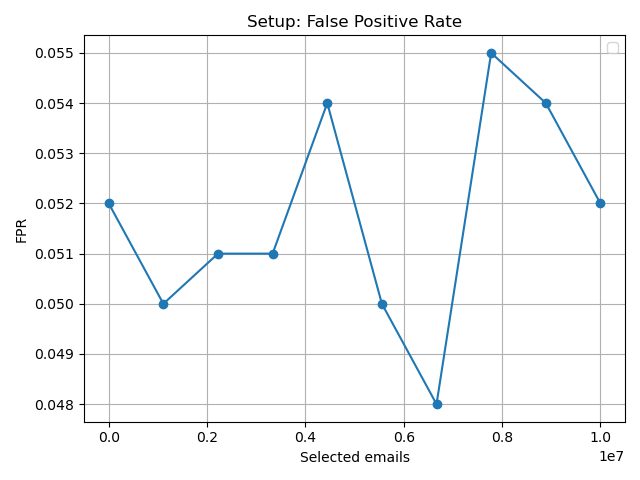
\includegraphics[width=\linewidth]{openmp/005/setup_fpr}
        \caption{FPR setup Omp}\label{fig:005-setup_fpr_omp}
    \endminipage\hfill
\end{figure}

\subsubsection{Filter}\label{subsubsec:fpr-005-filter}
\begin{figure}[H]
    \centering
    \minipage{0.49\textwidth}
    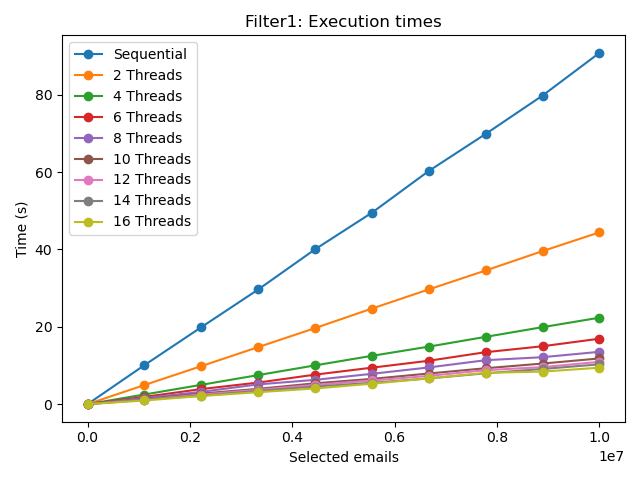
\includegraphics[width=\linewidth]{openmp/005/filter1_times}
        \caption{Time Filter Omp}\label{fig:005-filter_time_omp}
    \endminipage\hfill
    \minipage{0.49\textwidth}
    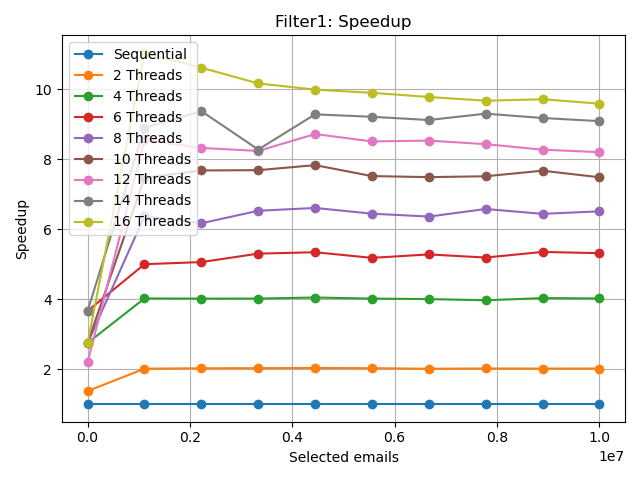
\includegraphics[width=\linewidth]{openmp/005/filter1_speedup}
        \caption{Speedup Filter Omp}\label{fig:005-filter_speedup_omp}
    \endminipage\hfill
\end{figure}
\begin{figure}[H]
    \centering
    \minipage{0.49\textwidth}
    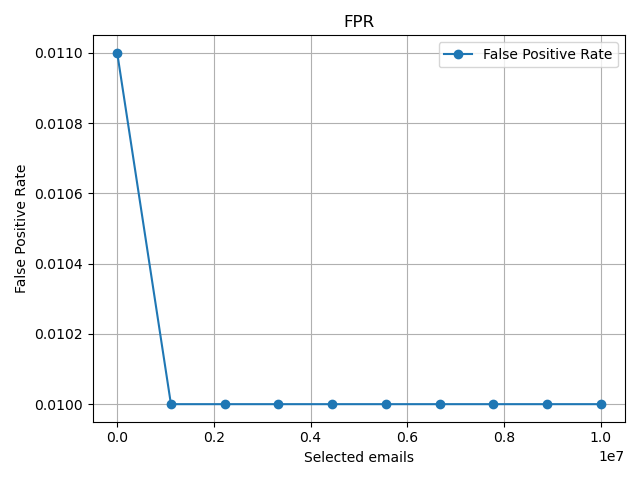
\includegraphics[width=\linewidth]{openmp/005/filter_fpr}
        \caption{FPR Filter Omp}\label{fig:005-filter_fpr_omp}
    \endminipage\hfill
\end{figure}


\subsection{Joblib}\label{subsec:joblib-test}
\subsubsection{Setup}\label{subsubsec:joblib-setup}
\begin{figure}[H]
    \centering
    \minipage{0.49\textwidth}
    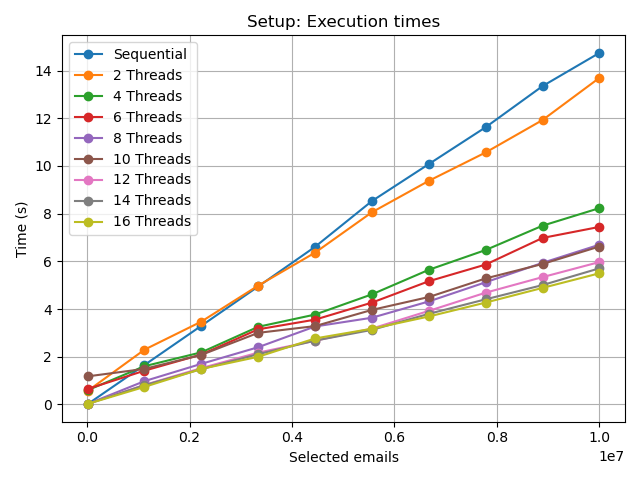
\includegraphics[width=\linewidth]{joblib/005/setup_time_plot}
        \caption{Time setup Joblib}\label{fig:005-setup_time_joblib}
    \endminipage\hfill
    \minipage{0.49\textwidth}
    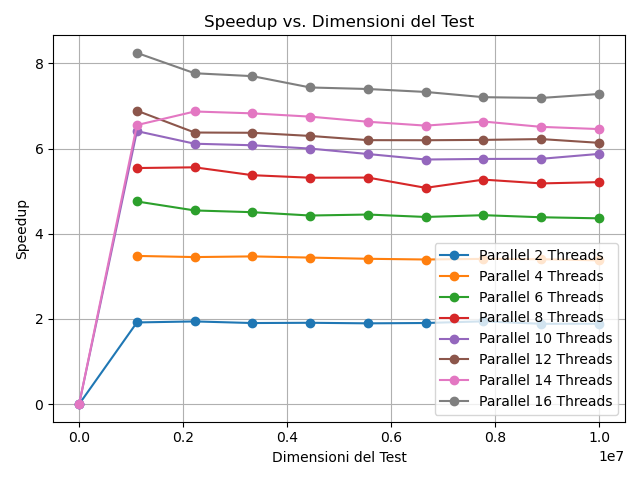
\includegraphics[width=\linewidth]{joblib/005/setup_speedup_plot}
        \caption{Speedup setup Joblib}\label{fig:005-setup_speedup_joblib}
    \endminipage\hfill
\end{figure}
\begin{figure}[H]
    \centering
    \minipage{0.49\textwidth}
    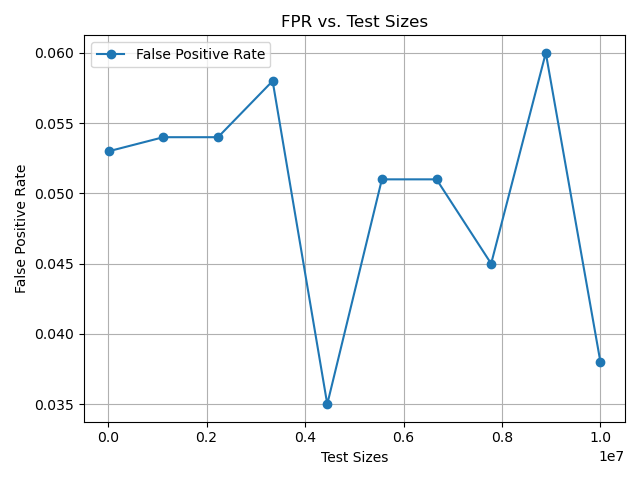
\includegraphics[width=\linewidth]{joblib/005/setup_fpr_plot}
        \caption{FPR setup Joblib}\label{fig:005-setup_fpr_joblib}
    \endminipage\hfill
\end{figure}

\subsubsection{Filter}\label{subsubsec:joblib-filter}
\begin{figure}
    \centering
    \minipage{0.49\textwidth}
    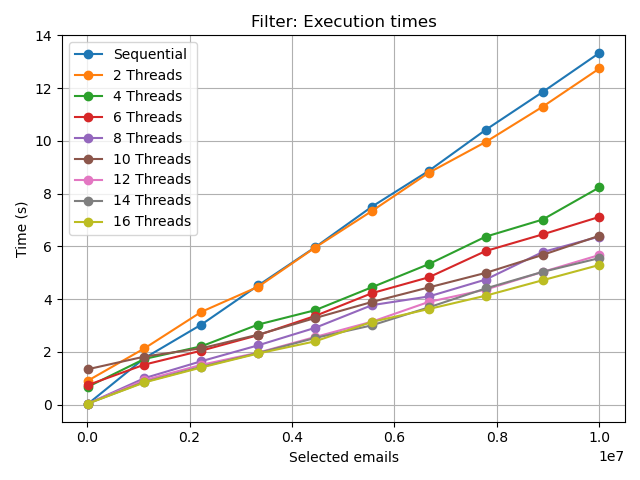
\includegraphics[width=\linewidth]{joblib/005/filter_time_plot}
        \caption{Time Filter Joblib}\label{fig:005-filter_time_joblib}
    \endminipage\hfill
    \minipage{0.49\textwidth}
    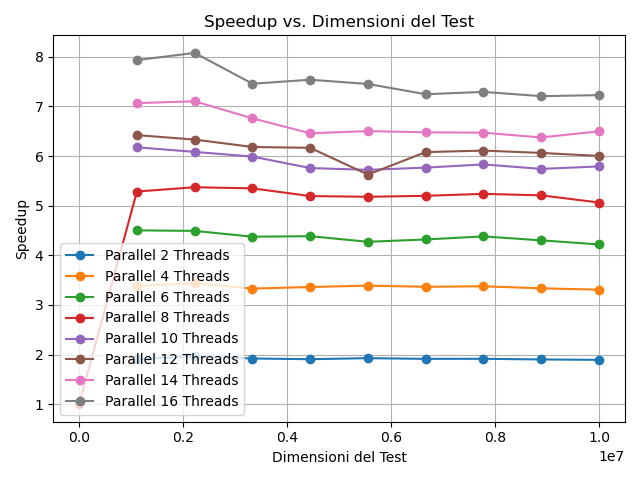
\includegraphics[width=\linewidth]{joblib/005/filter_speedup_plot}
        \caption{Speedup Filter Joblib}\label{fig:005-filter_speedup_joblib}
    \endminipage\hfill
\end{figure}
\begin{figure}[H]
    \centering
    \minipage{0.49\textwidth}
    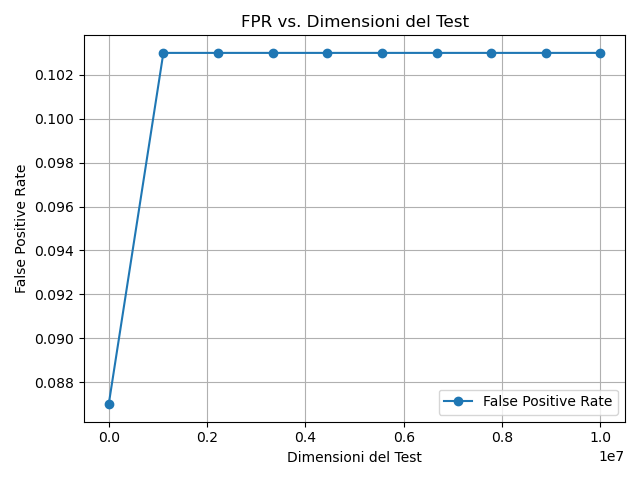
\includegraphics[width=\linewidth]{joblib/005/filter_fpr_plot}
        \caption{FPR Filter Joblib}\label{fig:005-filter_fpr_joblib}
    \endminipage\hfill
\end{figure}

\subsubsection{Chunks}\label{subsubsec:005-chunks}
Esploriamo ora l'opzione di eseguire un'operazione di chunking più ampia rispetto al numero di thread disponibili per
verificare se è possibile migliorare le performance, focalizzandoci esclusivamente sulla versione Joblib.
I valori di riferimento per i chunks sono 16, 32, 64, 128, 256, 512, 1024, 2048.

\begin{figure}[H]
    \centering
    \minipage{0.49\textwidth}
    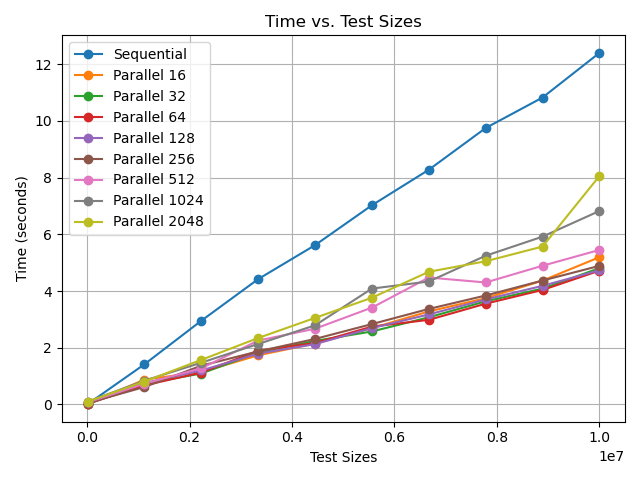
\includegraphics[width=\linewidth]{joblib/005/chunks_time_plot}
        \caption{Times setup Chunks}\label{fig:005-chunks_time}
    \endminipage\hfill
    \minipage{0.49\textwidth}
    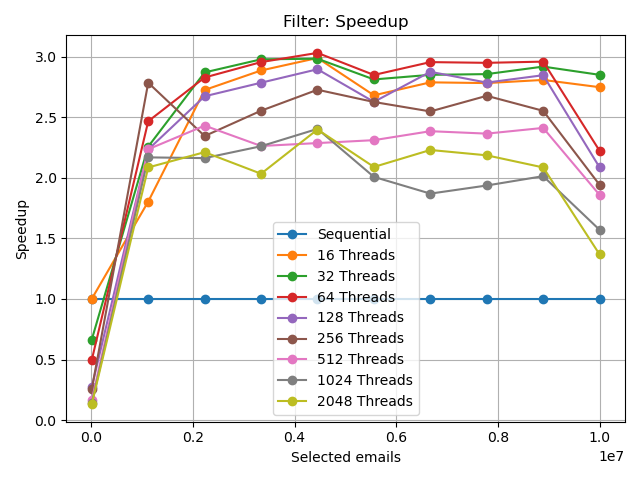
\includegraphics[width=\linewidth]{joblib/005/chunks_speedup_plot}
        \caption{Speedup setup Chunks}\label{fig:005-chunks_speedup}
    \endminipage\hfill
\end{figure}

I risultati ottenuti indicano che l'applicazione dell'operazione di chunking ha determinato miglioramenti
significativi nelle performance di speedup.
In particolare, l'aumento del numero di chunk ha contribuito a un miglioramento dello speedup,
raggiungendo un massimo di 3.
Tuttavia, oltre una soglia di 64 chunk, si è verificato un declino nelle performance.


\subsection{Confronto}\label{subsec:confronto}
Per il test di configurazione iniziale, è evidente che la versione sviluppata con OpenMP presenta una performance
temporale inferiore rispetto alla controparte.
Al contrario, in termini di speedup, la versione OpenMP supera la versione sviluppata con Joblib,
raggiungendo uno speedup massimo di 2.70 nella versione Joblib e 9 nella versione OpenMP, utilizzando il massimo
numero di thread disponibili.

I risultati massimi sono stati ottenuti sfruttando il numero massimo di thread disponibili.
Nel contesto della versione Joblib, i test iniziali con un numero più elevato di thread mostrano un tempo di esecuzione
peggiore rispetto alla versione sequenziale, probabilmente a causa del tempo di inizializzazione dei thread.
Nonostante l'aumento del numero di thread nella versione Joblib, lo speedup si stabilizza intorno al valore di 2.

Va notato che i valori di FPR (False Positive Rate) sono molto simili tra le due versioni.


Per il test di filtraggio, è evidente che la versione sviluppata con OpenMP presenta una performance temporale
inferiore rispetto alla sua controparte.
Tuttavia, in termini di speedup, la versione OpenMP supera la versione sviluppata con Joblib, raggiungendo un
massimo di 11 nella versione OpenMP e 2.5 nella versione Joblib, sfruttando il massimo numero di thread disponibili.

Anche in questo contesto, i valori di FPR (False Positive Rate) sono praticamente identici tra le due versioni.



